\documentclass[tikz,border=2pt]{standalone}
\usepackage{amsmath,amssymb}
\usepackage{tikz}
\usetikzlibrary{arrows.meta}

\begin{document}
% Sensitivity analysis asks how far the data may change before the answer changes: tilting
% the objective within the cone at the optimal corner keeps (20, 60) optimal; shifting a
% binding constraint moves the corner but keeps the same basis.
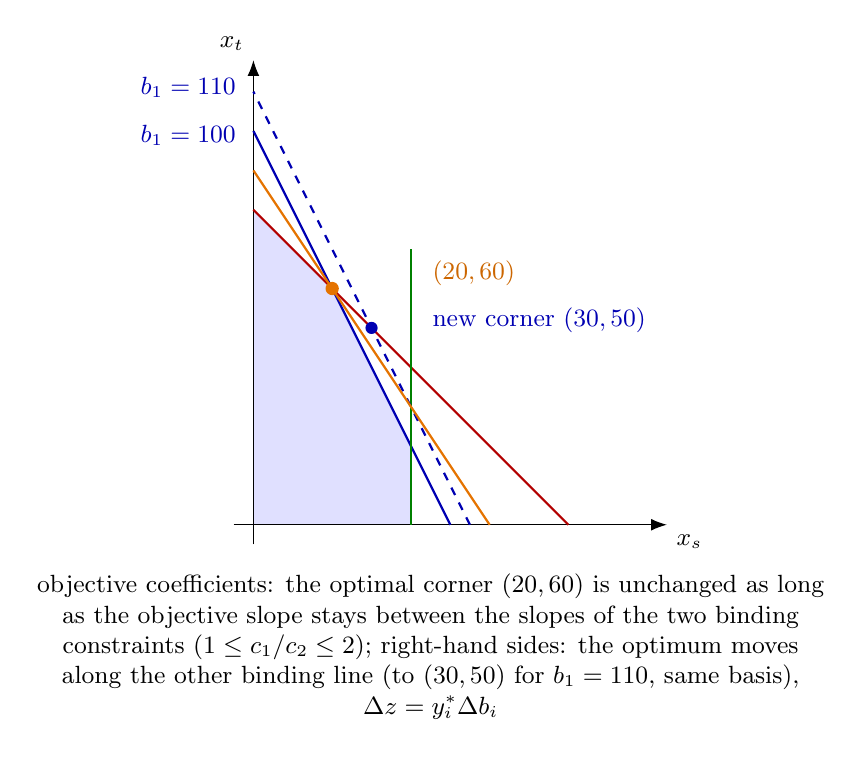
\begin{tikzpicture}[x=0.05cm, y=0.05cm, every node/.style={font=\small}, >={Latex[length=2mm]}]
	\fill[blue!12] (0,0) -- (40,0) -- (40,20) -- (20,60) -- (0,80) -- cycle;
	\draw[->] (-5,0) -- (105,0) node[below right] {$x_s$};
	\draw[->] (0,-5) -- (0,118) node[above left] {$x_t$};
	\draw[blue!70!black, thick] (50,0) -- (0,100);
	\draw[red!70!black, thick] (80,0) -- (0,80);
	\draw[green!50!black, thick] (40,0) -- (40,70);
	\draw[blue!70!black, thick, dashed] (55,0) -- (0,110);
	\node[blue!70!black, font=\small, anchor=east] at (-2,111) {$b_1=110$};
	\node[blue!70!black, font=\small, anchor=east] at (-2,99) {$b_1=100$};
	\draw[orange!90!black, thick] (60,0) -- (0,90);
	\fill[orange!90!black] (20,60) circle (2.4pt);
	\fill[blue!70!black] (30,50) circle (2.2pt);
	\node[orange!80!black, font=\small, anchor=west] at (43,64) {$(20,60)$};
	\node[blue!70!black, font=\small, anchor=west] at (43,52) {new corner $(30,50)$};
	\node[anchor=north, align=flush center, text width=10cm] at (45,-10) {objective coefficients: the optimal corner $(20,60)$ is unchanged as long as the objective slope stays between the slopes of the two binding constraints ($1\le c_1/c_2\le2$); right-hand sides: the optimum moves along the other binding line (to $(30,50)$ for $b_1=110$, same basis), $\Delta z=y_i^\ast\Delta b_i$};
\end{tikzpicture}
\end{document}
